
\chapter{Pruebas de funcionamiento}

Para revisar el buen funcionamiento de la aplicación desarrollada, se utilizaró el software dispuesto por Apple Inc,  el entorno de desarrollo Xcode y herramientas asociadas. Para obtener estas aplicaciones, es necesario poseer una cuenta de desarrollador para \textbf{iOS} o \textbf{Mac OS X}, las cuales se pueden obtener en el sitio web \url{https://developer.apple.com/programs/} luego de pagar la matrícula impuesta.\\

La cuenta de desarrollador permite acceso al repositorio de herramientas \cite{apple-repositorio} y también acceso a versiones de los sistemas operativos antes de lanzamiento.
Además permite poner a la venta las aplicaciones desarrolladas en la \textit{\textbf{App Store}}\cite{apple-appstore}.

% datos en el camino, seguimiento de un tweet, pantallazos de debug
\section{Cambio de tiempo y/o canal}

Las primeras pruebas estuvieron relacionadas con el cambio de tiempo a través de peticiones al dispatcher con argumentos en la cadena de consulta, estas se realizaron con la aplicación de OS X: \textbf{Quicktime X}, la cual permite reproducir streams que cumplen con las espeficicaciones de HTTP Live Streaming. Otra alternativa que además se encuentra disponible en otros sistemas operativos es \textbf{VideoLan VLC}. Las pruebas consistieron en modificar los argumentos \textbf{t}, \textbf{s} y \textbf{c} de URLs del tipo:
\url{http://ssdemo.altavoz.net/playlist/playlist.m3u8?s=tvn&t=1353186024&c=0}, donde el parámetro \textbf{t} corresponde al tiempo Unix del 17 de noviembre de 2012 18:00:24 GMT-3.\\

El escificar el tiempo en el parámetro \textbf{t} resulta siempre en una lista de reproducción con segmentos asociados al tiempo correspondiente. Además se monitoreó la respuesta a través de la aplicación rastreadora de paquetes Wireshark. Para esto se necesitó aplicar un filtro especial de forma que los paquetes relacionados con HTTP Live Streaming fueran entregados. El filtro corresponde a mostrar paquetes recibidos desde el servidor donde el cliente, en este caso Quicktime, se contacta para obtener una lista de reproducción, y además pedir la entrega de paquetes que tengan en su contenido la palabra \textbf{apple}.

\begin{figure}[H]
	\centering
\begin{lstlisting}
		ip.addr==200.91.44.49 && http contains apple
\end{lstlisting}
\caption{Filtro en Wireshark que muestra sólo paquetes relacionados con el HLS}
\end{figure}


Los resultados obtenidos son los esperados y corresponden a la reproducción del video en el momento indicado y en el canal indicado según los parámetros.

\begin{figure}[H]
	\centering
	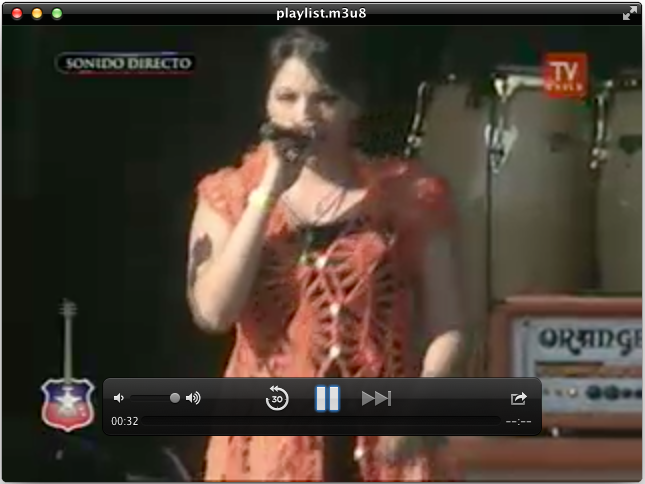
\includegraphics[scale=0.5]{imgs/qt-tvn.png}
	\caption{Captura de Quicktime reproduciendo lista de reproducción a través de un URL.}
	\label{qt-tvn}	
\end{figure}

\begin{figure}[H]
	\centering
	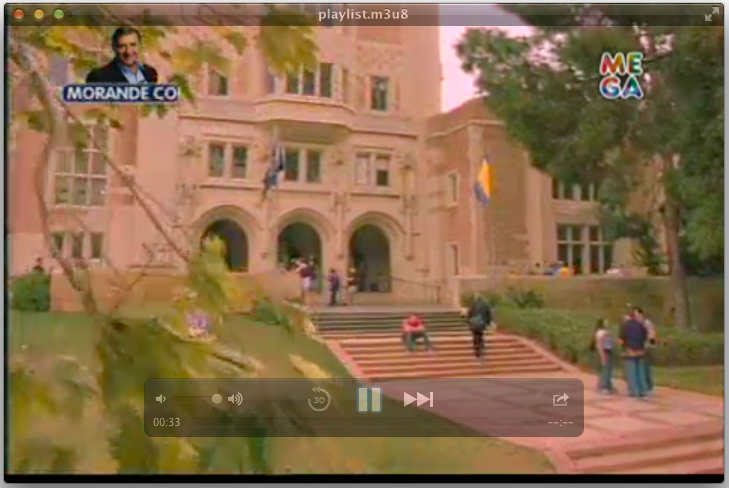
\includegraphics[scale=0.5]{imgs/qt-mega.png}
	\caption{}
	\label{qt-mega}	
\end{figure}

\begin{figure}[H]
	\centering
	\begin{tabular}{cc}
	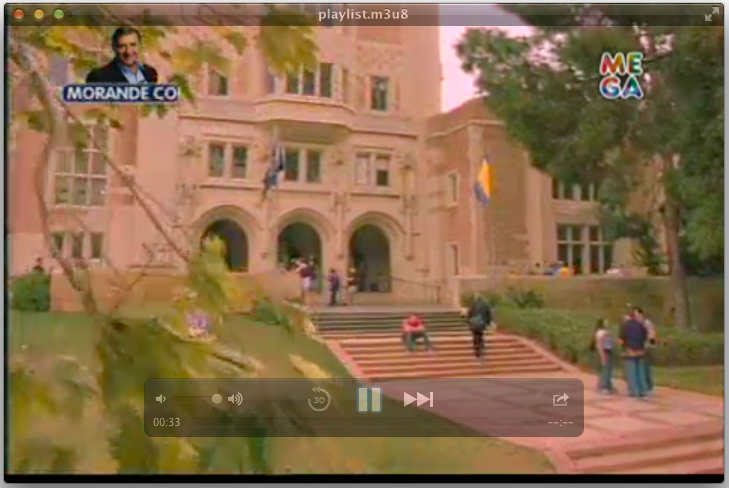
\includegraphics[scale=0.3]{imgs/qt-mega.png} & 
	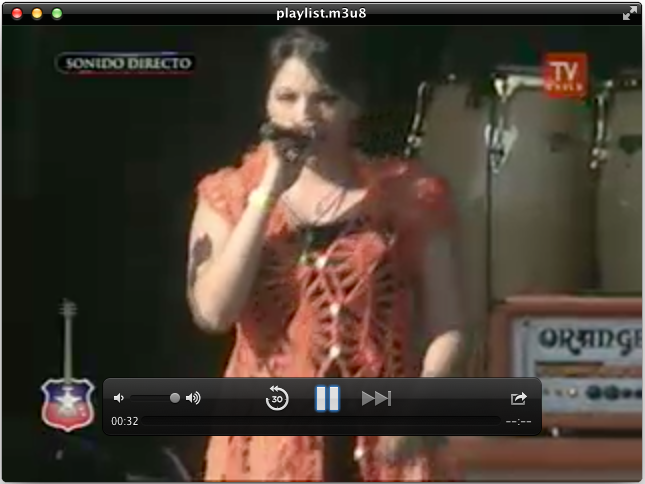
\includegraphics[scale=0.3]{imgs/qt-tvn.png} \\
	\end{tabular}
	\caption{Captura de Quicktime reproduciendo lista de reproducción a través de un URL.}
	\label{qt-tvn-mega}
\end{figure}

%http://ssdemo.altavoz.net/playlist/playlist.m3u8?s=tvn&t=1353186024&c=0
%http://ssdemo.altavoz.net/playlist/playlist.m3u8?s=video1&t=1353186024&c=0

%escribir en consola el URL, probarlo en quicktime, vlc, navegador, app, wireshark para ver cookies

\section{Proceso corriendo en fondo} % background

escribir en consola los seekable time ranges, poner pausa background y al retomar reproducir, se notó que avanzaba la lista de iguañl forma. se arregó guardando la fecha al momento de poner pausa. que se llamaba al irse a background.

\section{Cambio de ancho de banda}

se especifica requerimiento a la empresa, se modifica el dispatcher con lista de variantes, se revisa en wireshark.
luego se utiliza la herramienta network link conditioner para modificar el BW en plena transmisión, revisar wireshark cuando cambia y ver en la misma app.
Luego se prueba con iPhone cambiando entre wifi y 3g

  \subsection{WiFi}
  se agrega campo en el URL para priorizar distintas variantes, con wifi video, 3g audio.
  \subsection{3G}
  con 3g 
\section{Cambio de transmisión mediante Twitter}
- se revisa usando safari desktop con script que incluye player


  \subsection{Dentro de la aplicación}
	- debug viendo el cambio de tranmisión, URL generado y definiendo el mismo canal. manejo en caso de tweet sin enlace
  \subsection{Scheme registrado en iOS}
	- clientes de twitter en iPhone, twitter y Tweetbot, debug en el método e imprimir en consola la app que lo lanzó.  
	- debug con app en background
	- debug con app cerrada y a la espera que parta por otra aplicación
  
\section{Enlaces Twitter en otros dispositivos}
	pantallazos de páginas de error, el por qué y cómo se entregan según el script
  \subsection{PC Escritorio}
    \subsubsection{Chrome}
    foto
    \subsubsection{Safari}
    foto del player
    \subsubsection{Firefox}
    foto
    \subsubsection{Opera}
    foto
    \subsubsection{Internet Explorer}
    foto
  \subsection{Android y otros móviles incompatibles}
  pantallazo del cell de la esperanza
\section{Comparación con SocialStream Flash}
mostrar player original de eduardo, la diferencia de la linea de tiempo, el salto de tiempo, la exactitud y que no es tan exacto porque los segmentos son de 10 segundos
